\section{Streaming-rANS}

% Add outline page for Introduction section
\begin{frame}{Outline}
    \tableofcontents[
        currentsection, 
        sectionstyle=show/hide, 
        subsectionstyle=show/show/hide, 
        subsubsectionstyle=show/show/show]
\end{frame}

    \begin{frame}[fragile]{Streaming-rANS}
        To avoid using large number arithmetic, in practice stream variants are used: which enforce by renormalization: sending the least significant bits of x to or from the bitstream (usually L and b are powers of 2). \refer{4}
    \end{frame}

\subsection{Problem}
    \begin{frame}
        Example of the problem //TODO: add example
    \end{frame}
    \begin{frame}
        \begin{itemize}
            \item ANS (Asymmetric Numeral Systems) uses a single integer x, known as the “state,” to represent the encoded data.
            \item Over time, as more symbols are encoded, the state x can grow arbitrarily large. This can lead to:
            \begin{itemize}
                \item Overflow: If the value exceeds the precision limits of your system (e.g., a 32-bit or 64-bit register).
                \item Inefficient Encoding: A larger x means you need more memory or bits to represent it.
            \end{itemize}
            \item Using the C function from the previous section to encode succeeding symbols, we can encode a sequence into a very large natural number $\mathit{x}$, which can be stored as a length $\mathit{\lfloor lg(x) \rfloor+ 1}$ bit sequence. \refer{2}
        \end{itemize}
    \end{frame}

\subsection{Idea}
\begin{frame}[fragile]{Renormalization in Range Coding}
    \begin{itemize}
        \item Range Coding
        \begin{itemize}
            \item 1
            \item 2
        \end{itemize}
        \item we use the similar idea for rANS
        \begin{itemize}
            \item range $\mathit{[L, H]}$
            \item Encoding: shrink the current state $\mathit{x}$ until it is in the range $\mathit{[L, H]}$ 
            \item Decoding: expand the current state $\mathit{x}$ until it is in the range $\mathit{[L, H]}$
        \end{itemize}
        \item In AC, renormalization is used to allow finite precision, an analogous approach should be used for ANS. Specifically, we will enforce xto remain in some fixed range I by transferring the least significant bits to the stream. For generality, let us transfer a base $\mathit{b}$ digit, for example $\mathit{b}= 2$ means transferring single bits, while $\mathit{b} = 2^8$ means transferring complete bytes.
    \end{itemize}
\end{frame}

\subsection{Solution}
\subsubsection{Renormalization}
\begin{frame}[fragile]{Methods from Jarek Duda: Method 1 - Decoding \refer{2}}
    \pseudo{ANS decoding step from state $x$}{
        $\mathit{(s, x) = D(x)}$ \textcolor{gray}{\fontsize{9}{12}\selectfont\textit{\# decode the current state x}} \\
        useSymbol($\mathit{s}$) \\
        \textbf{while} $\mathit{x < \textcolor{red}{L}}$ \textbf{do} \textcolor{gray}{\fontsize{9}{12}\selectfont\textit{\# if x is too small that not in the range [L,H]}}\\
        \quad \textcolor{gray}{\fontsize{9}{12}\selectfont\textit{\# expand the x by reading the outstreamed digits back from the stream (an array)}}\\
        \quad $\mathit{\text{expand}(x,b) = b \cdot x + \text{readDigit}()} \rightarrow \mathit{x}$\\
        \textbf{end while} \\
        \textcolor{gray}{\fontsize{9}{12}\selectfont\textit{\# return the new state}}
    }
\end{frame}
\begin{frame}[fragile]{\textcolor{red}{What is $\mathit{L,H}$ ?}}
    \begin{center}
        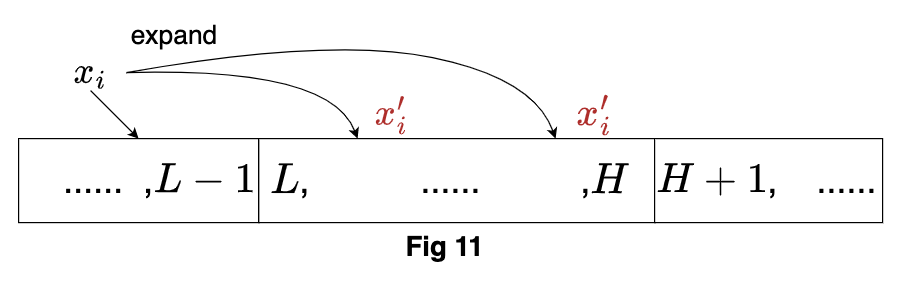
\includegraphics[width=0.8\textwidth,keepaspectratio]{../24ws_ANS.assets/fig11.png}
    \end{center}
\end{frame}
\begin{frame}[fragile]{\textcolor{red}{What is $\mathit{L,H}$ ?}}
    \begin{itemize}
        \item $\mathit{x_i = b \cdot x_{i-1} + \text{bit}}$
        \item Either $\mathit{x_i}$ in $\mathit{[L, H]}$ or $\mathit{x_{i-1}}$ in $\mathit{[L, H]}$. Assume $\mathit{x_{i-1}}$ in $\mathit{[L, H]}$.
            \begin{itemize}
                \item $\mathit{x_{i-1} >= L}$
                \item $\mathit{x_i >= b \cdot L + bit >= b \cdot L}$
                \item $\mathit{x_i}$ can't be in $\mathit{[L, H]}$
                \item derive: $\mathit{H <= b\cdot L -1}$
            \end{itemize}
        \item $\mathit{[L,H]}$, where $\mathit{H <= b\cdot L -1}$ \textcolor{blue}{(Constraint 1)}
        \item $\mathit{I=\{L, ..., b\cdot L -1\}}$, which is defined by Jarek Duda \textbf{$\mathit{b}$-unique interval} and $\mathit{L \in \mathbb{N}}$
        \item This will ensure that the loop in Method 1 will always return to the original value
    \end{itemize}
\end{frame}
\begin{frame}[fragile]{Methods from Jarek Duda: Method 2 - Encoding \refer{2}}
    shrink the current state $\mathit{x}$ by stream out the least significant bit ($\mathit{x}$ will be stored in binary and we take out the bit from right side)
    \pseudo{ANS encoding step of symbol sfrom state $\mathit{x}$}{
        \textcolor{gray}{\fontsize{9}{12}\selectfont\textit{\# once the current state x is greater than max value that we define later}} \\
        \textbf{while} $\mathit{x > \textcolor{red}{maxX[s]}}$ \textbf{do}\\
        \quad \textcolor{gray}{\fontsize{9}{12}\selectfont\textit{\# write the least significant digit to the stream (stream could be an array in implementaion )}} \\
        \quad writeDigit(mod($\mathit{x,b}$)) \\
        \quad $\mathit{\text{shrink}(x,b)=\lfloor x/b \rfloor \rightarrow x}$ \textcolor{gray}{\fontsize{9}{12}\selectfont\textit{\# shrink the x}}\\
        \textbf{end while} \\
        $\mathit{x=C(s,x)}$ \textcolor{gray}{\fontsize{9}{12}\selectfont\textit{\# encode with the shrunk x}}
    }
\end{frame}
\begin{frame}[fragile]{\textcolor{red}{What is $\mathit{maxX[s]}$?}}
    \begin{center}
        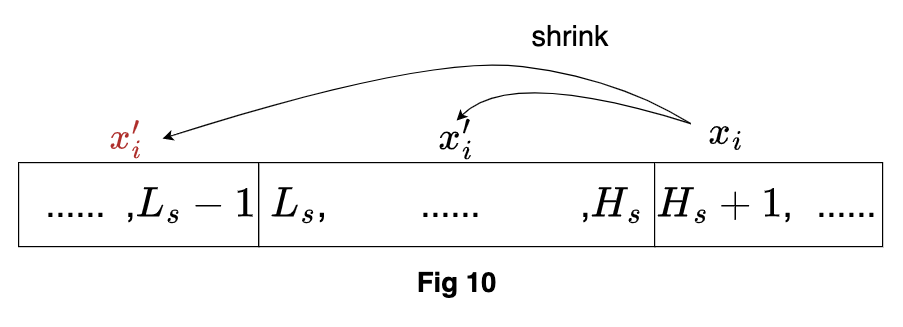
\includegraphics[width=0.8\textwidth,keepaspectratio]{../24ws_ANS.assets/fig10.png}
    \end{center}
\end{frame}
\begin{frame}[fragile]{\textcolor{red}{What is $\mathit{maxX[s]}$?}}
    \begin{itemize}
        \item to make sure not to jump over the range
        \item Assume that $\mathit{x_i = H_s + 1}$ and it will be shrinked to $\mathit{x_i'=\lfloor x_i/b \rfloor}$
        \item $\mathit{x_i' = \lfloor x_i/b \rfloor = \lfloor (H_s + 1)/b \rfloor >= L_s}$
        \item $\mathit{ L_s <= (H_s + 1) / b <= \lfloor (H_s + 1)/b \rfloor < (H_s + 1)/b + 1}$
        \item $\mathit{H_s >= b \cdot L_s - 1}$, $\forall \mathit{s} \in \mathcal{A}$ \textcolor{blue}{(Constraint 2)}
    \end{itemize}
\end{frame}
\begin{frame}[fragile]{Final Form of $[L,H]$ in practice}
    \begin{itemize}
        \item Contraints $$\begin{gathered}\mathit{[L,H]}: \text{ where } \mathit{H <= b\cdot L -1} \\ \mathit{[L_s, H_s]: H_s >= b \cdot L_s - 1}, \forall \mathit{s} \in \mathcal{A}\end{gathered}$$
        \item In practice ($\mathit{b}=2^1$): we choose $\mathit{L=k\cdot m}$, $\mathit{L_s=k\cdot F_s}$ ($\mathit{k} \in \mathbb{N}$) $$\begin{gathered}\mathcal{I}=\mathit{[km}, 2\cdot \mathit{km}-1] \\ \mathcal{I}_{\mathit{s}} =[\mathit{kF_s}, \,2\cdot \mathit{kF_s} -1] \text{   for   } \forall \mathit{s} \in \mathcal{A} \end{gathered}$$
    \end{itemize}
\end{frame}

\subsection{Implementation of Streaming-rANS}
\subsubsection{Encoding}
\begin{frame}[fragile]
    \href{http://localhost:8050}{implementation with python} (\href{https://github.com/hurryclear/cs_theory/tree/data_compression/24ws_data_compression/implementation}{dash app})
    \begin{minted}[fontsize=\scriptsize, linenos, breaklines]{python}
    def rANS_stream_encoder(symbol_counts, s_input):
        # Init: c_s, m, x, output, bit_stream (omit the code here)
        for s in s_input:
            F_s = symbol_counts[s]
            c_s = cumul_freq[s]
            L_s = F_s # k = 1
            maxX_s = 2 * L_s - 1
            out_bits = ""

            while x > maxX_s:
                out_bits += str(x % 2)
                x = x // 2
            x = (x // F_s) * sum_freq + (x % F_s) + c_s
            bit_stream += out_bits
            output.append((s, x, out_bits, bit_stream))
        
        return output, x, bit_stream, L_avg, entropy(symbol_counts)
    \end{minted}
\end{frame}
\subsubsection{Dncoding}
\begin{frame}[fragile]
    \href{http://localhost:8050}{implementation with python} (\href{https://github.com/hurryclear/cs_theory/tree/data_compression/24ws_data_compression/implementation}{dash app})
    \begin{minted}[fontsize=\scriptsize, linenos, breaklines]{python}
    def rANS_stream_decoder(symbol_counts, x, bit_stream, num_symbols):
        # Init: c_s, m, x, output, bit_stream (omit the code here)
        bit_stream = list(map(int, bit_stream.split(',')))  # Convert bit_stream to a list of integers
        for _ in range(num_symbols):
            slot = x % sum_freq
            s = bisect_right(cumul_freq, slot) - 1
            F_s = symbol_counts[s]
            c_s = cumul_freq[s]
            output.append((s, x))
            x = (x // sum_freq) * F_s + slot - c_s

            while x < sum_freq and len(bit_stream) > 0: 
                x = x * 2 + bit_stream.pop()
        
        return output, x
    \end{minted}
\end{frame}